\subsection{Counter}

\begin{figure}[htbp]
   \centering
   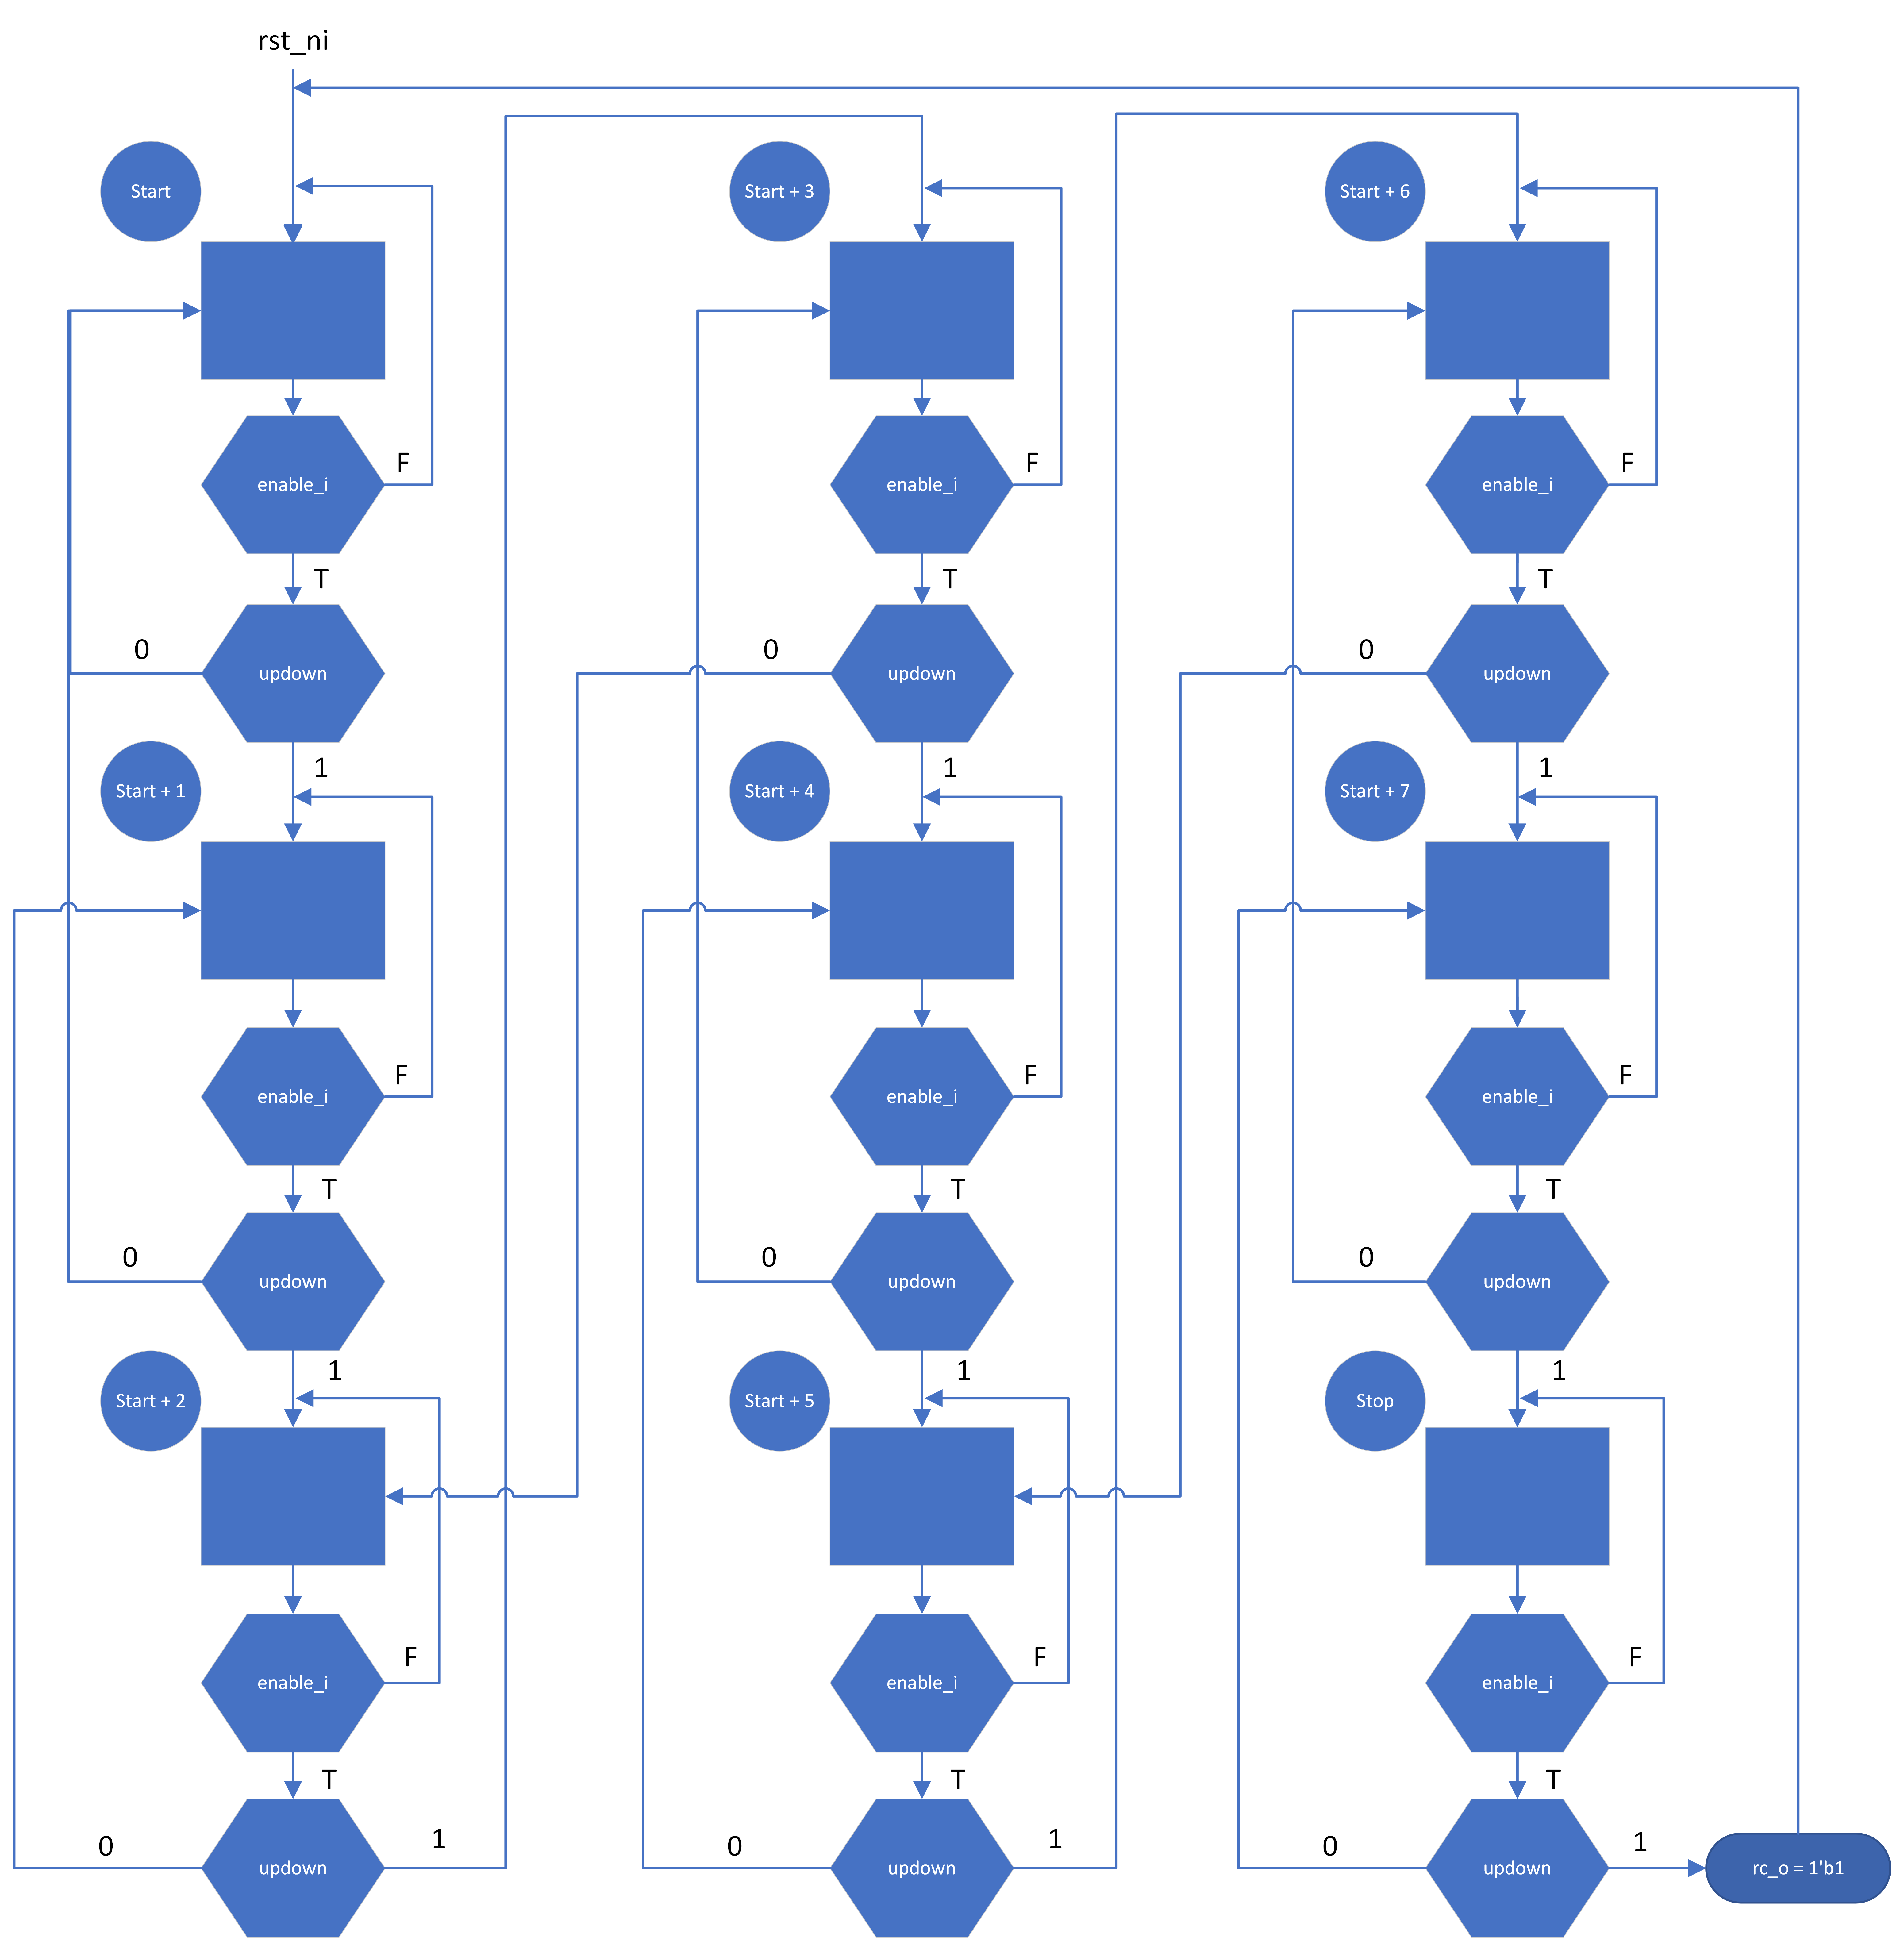
\includegraphics[width=\textwidth]{counter_asm.png}
   \caption{ASM chart of the counter module.}
   \label{fig:counter_asm}
\end{figure}

\begin{minted}[
   fontsize=\footnotesize,
   linenos,
   breaklines,
]{verilog}
module counter (
   input clk_i,
   input rst_ni,
   input updown_i,
   input enable_i,
   output [3:0] bcd_o,
   output reg rc_o  // ripple carry output
);

reg [3:0] state_d, state_q;
assign bcd_o = state_q;

parameter Start = 4'b0000;
parameter Stop  = 4'b1001;

always @(posedge clk_i, negedge rst_ni)
   if (~rst_ni)
      state_q <= Start;
   else
      state_q <= state_d;

always @(state_q, enable_i, updown_i) begin
   rc_o = 1'b0;
   state_d = state_q;  // default assignment next state is present state
   if (enable_i)
      if (updown_i)  // count up
         if (state_d == Stop) begin
            state_d = Start;
            rc_o = 1'b1;
         end else
            state_d = state_d + 1'b1;
      else  // count down
         if (state_d == Start)
            state_d = Start;
         else
            state_d = state_d - 1'b1;
end

endmodule
\end{minted}

\begin{minted}[
   fontsize=\footnotesize,
   linenos,
   breaklines,
]{verilog}
module counter_tb;

// Inputs
reg clk;
reg rst_n;
reg updown_i;
reg enable_i;

// Outputs
wire [3:0] cnt_o;
wire ripple_carry_o;

counter DUT (
   .clk_i(clk),
   .rst_ni(rst_n),
   .updown_i(updown_i),
   .enable_i(enable_i),
   .bcd_o(cnt_o),
   .rc_o(ripple_carry_o)
);

// Create a 50Mhz clock
always #10 clk = !clk;  // every ten nanoseconds invert

initial begin
   clk = 1'b0;
   rst_n = 1'b0;
   enable_i = 1'b0;  // disabled
   updown_i = 1'b1;  // count up
end

initial begin
   #20 rst_n = 1'b1;  // release reset

   // Test count up and ripple carry generation
   repeat (11) begin
      @(posedge clk);
      enable_i = 1'b1;
      @(posedge clk);
      enable_i = 1'b0;
   end

   // Reset
   @(negedge clk);
   rst_n = 1'b0;
   @(negedge clk);
   rst_n = 1'b1;

   // Test count down
   repeat (9) begin
      @(posedge clk);
      enable_i = 1'b1;
      @(posedge clk);
      enable_i = 1'b0;
   end
   //updown_i = 1'b0;  // count down
   repeat (10) begin
      @(posedge clk);
      enable_i = 1'b1;
      updown_i = 1'b0;
      @(posedge clk);
      enable_i = 1'b0;
      updown_i = 1'b1;
   end

// Finish the Simulation
   #100;
   $finish;
end

endmodule
\end{minted}

\begin{figure}[htbp]
   \centering
   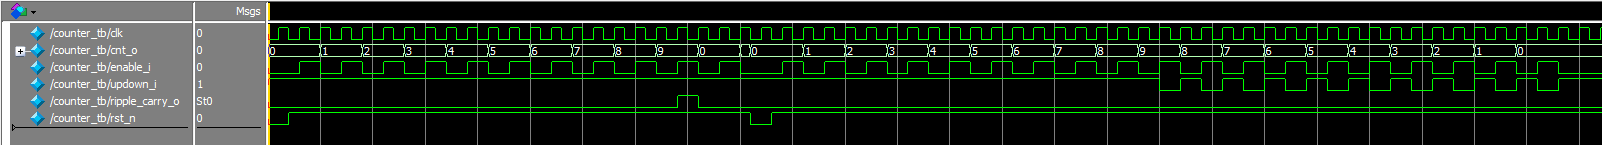
\includegraphics[width=\textwidth]{counter_sim.png}
   \caption{Testbench simulation of the counter module.}
   \label{fig:counter_sim}
\end{figure}

Fig.~\ref{fig:counter_sim} shows the simulation test results of the counter module. The counter counts up when updown is high potential and counts down when it is low potential. The enable signal triggers the counter to count once.

The first test case was to count from zero to nine. Nine set to the biggest digit this counter can count to. Counting once beyond nine returned the count to zero and generated a ripple carry. Next, Reset singal reset the count to zero. Then counting down was tested. Note that if count down to zero and then count down again, the count did not go back to nine but stayed at zero.
